
\chapter{Linear independence}

\index{linear independence}

One of the deepest and most central concepts in linear algebra -- in fact, if I
were to make a top ten ranking, this one might just make \#1 -- is that of
\textbf{linear independence}. It's not about mechanical computations, but
conceptual truths. Learn this chapter well. 

\section{The Domino Game}
\index{the Domino Game}

I've thought long and hard about the best way to teach the material in this
chapter, and I've come up with a game. I call it ``the Domino Game.'' Here are
the rules:

\begin{framed}
\begin{compactenum}
\item You are given one or more \textbf{yellow}\footnotemark ``starter dominoes.''
\item The object of the game is to build the white ``goal domino'' from these
starter dominoes.
\item You can ``use'' any number of each starter domino (even a fraction, even
negative), and add them together (left sides add together, and right sides add
together).
\item You \textit{cannot} use only one side of a domino.
\item You \textit{cannot} turn a domino around so the left side and right
sides flip.
\end{compactenum}
\end{framed}

\footnotetext{Light gray, actually, since I made this book black\&white to keep costs down.}

Example. Suppose your starter dominoes are:

\begin{center}
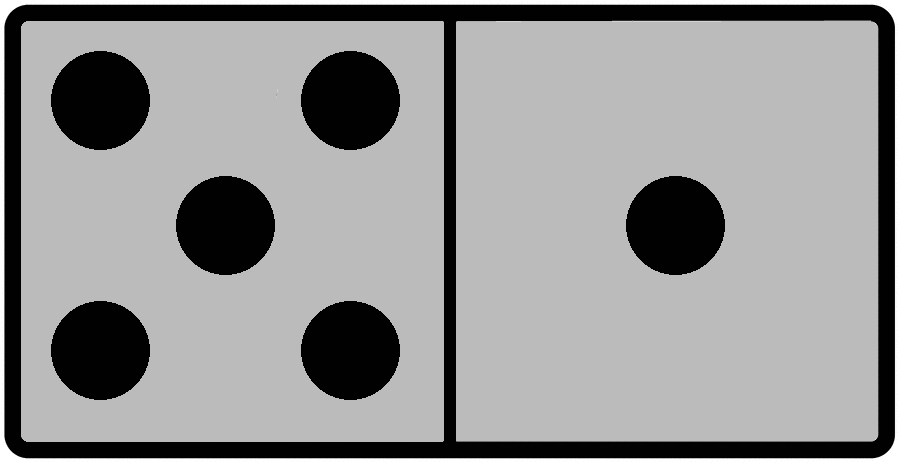
\includegraphics[width=0.3\textwidth]{gray5_1.png}
\hspace{.3in}
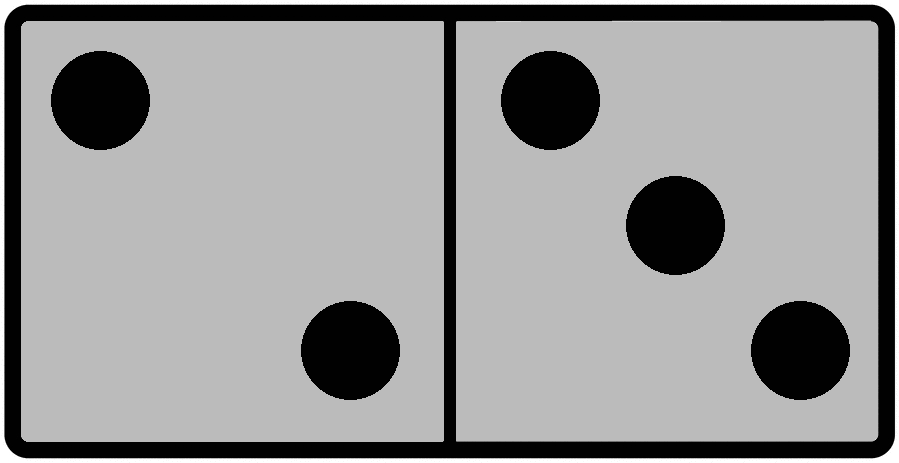
\includegraphics[width=0.3\textwidth]{gray2_3.png}
\end{center}

and your goal domino is:
\begin{center}
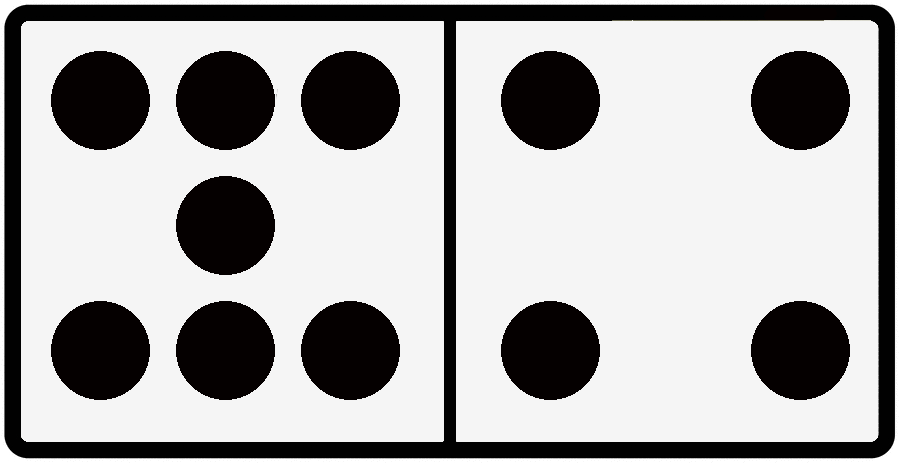
\includegraphics[width=0.3\textwidth]{white7_4.png}
\end{center}

A solution would be ``\textbf{one} and \textbf{one}.'' This means that you'll
take \textit{one} copy of the first starter domino, and \textit{one} copy of
the second, and add them together.

\begin{center}
{\LARGE Solution: \textbf{1 \& 1}}

1 \raisebox{-0.3\height}{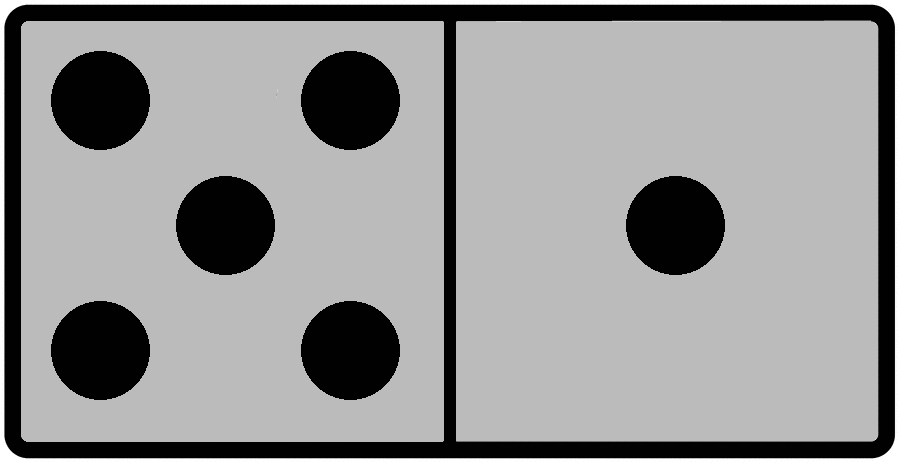
\includegraphics[width=0.1\textwidth]{gray5_1.png}} \ \& \
1 \raisebox{-0.3\height}{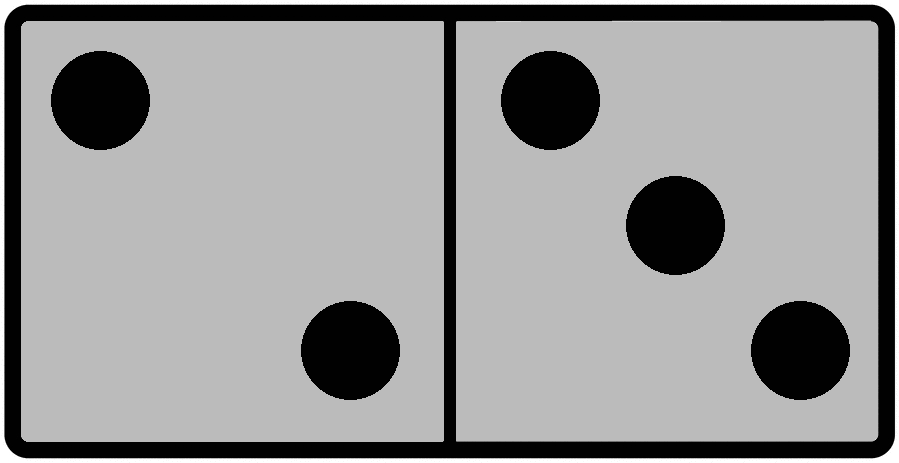
\includegraphics[width=0.1\textwidth]{gray2_3.png}} \ = \
\raisebox{-0.3\height}{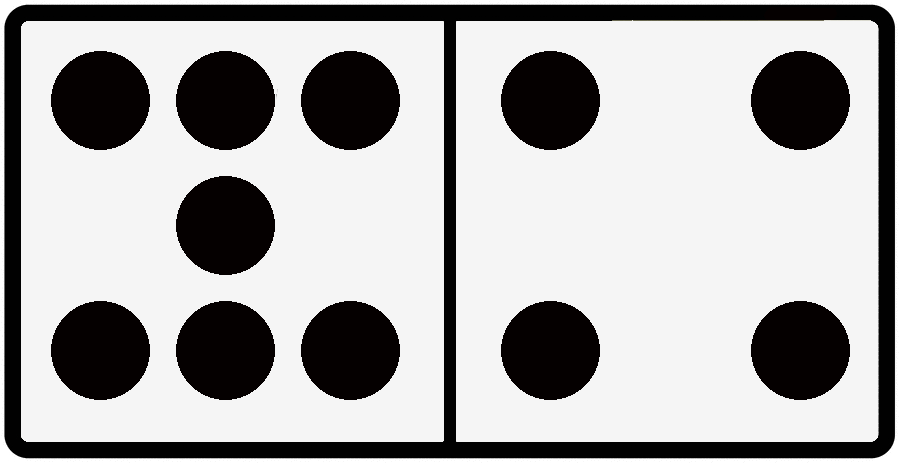
\includegraphics[width=0.1\textwidth]{white7_4.png}} \quad
\end{center}

Stare carefully at that until you master how it works; the rest of this chapter
will be a complete waste of time if this operation is not fully grasped. Adding
domino 5--1 to 2--3 means adding the left sides together, and separately adding
the right sides together, to produce a new domino 7--4 (since $5+2=7$ and
$1+3=4$).

\subsection{Actually do this}

All right, let's test your skillz. I want you to \textit{actually} work out the
answers to the following Domino Game puzzles on your own. There are six of
them, so it might take you a while (perhaps as long as 6 minutes). But it's
vital to cement your understanding of how this works...\textit{and} to set up
the crucial punchline later on in this chapter.

Answers to each puzzle are given at the end of the chapter. Maybe your answers
will not be the same as mine...or maybe they will? That itself is actually a
very important question we'll consider in a few minutes.

Enough preamble. Go!

\begin{enumerate}
\itemsep2em

\label{startDominoPuzzles}
\item Starter dominoes:
\hspace{.3in}
\raisebox{-0.3\height}{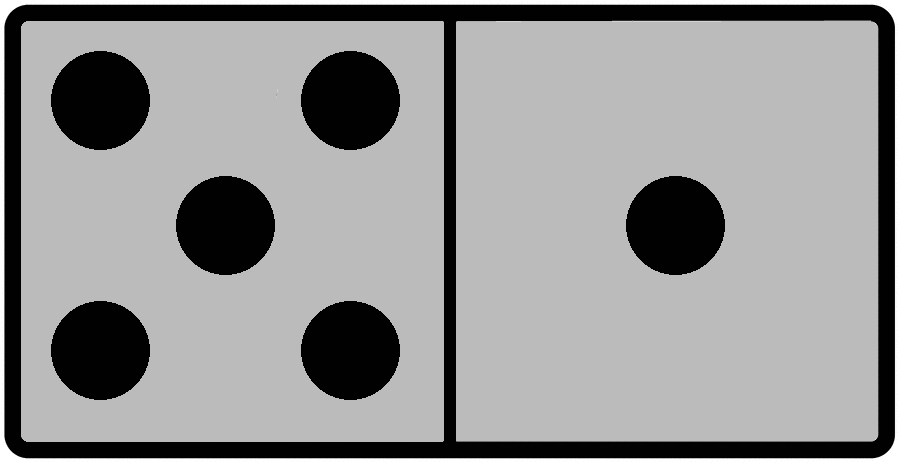
\includegraphics[width=0.2\textwidth]{gray5_1.png}}
\hspace{.1in}
\raisebox{-0.3\height}{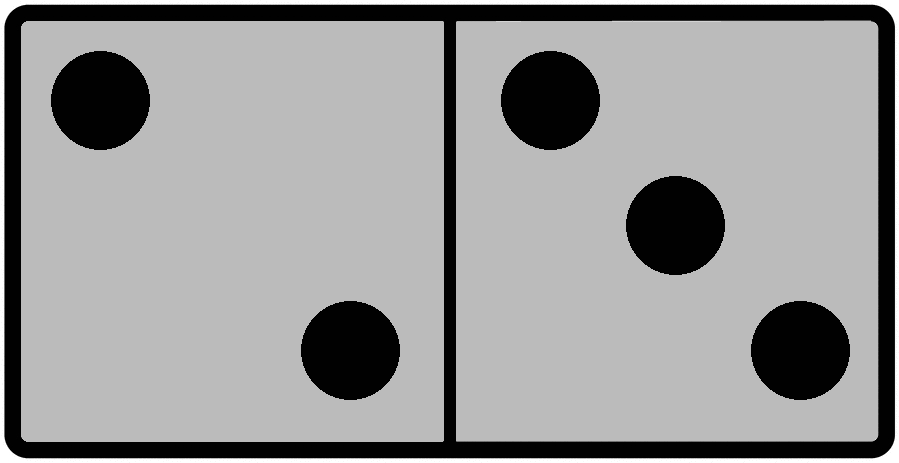
\includegraphics[width=0.2\textwidth]{gray2_3.png}}

Goal domino:
\hspace{1.1in}
\raisebox{-0.3\height}{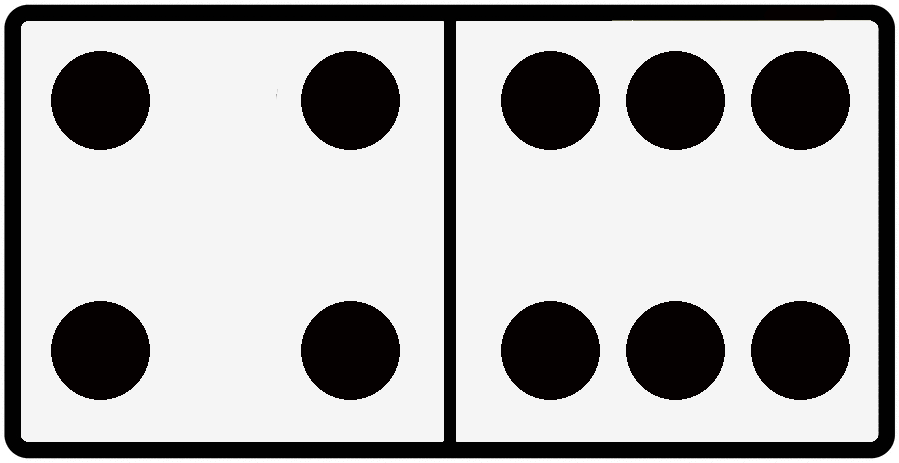
\includegraphics[width=0.2\textwidth]{white4_6.png}}

\footnotesize
(Hint: it's okay to take \textit{zero} of one of the dominoes; \textit{i.e.},
to completely ignore it.)
\normalsize

\item Starter dominoes:
\hspace{.3in}
\raisebox{-0.3\height}{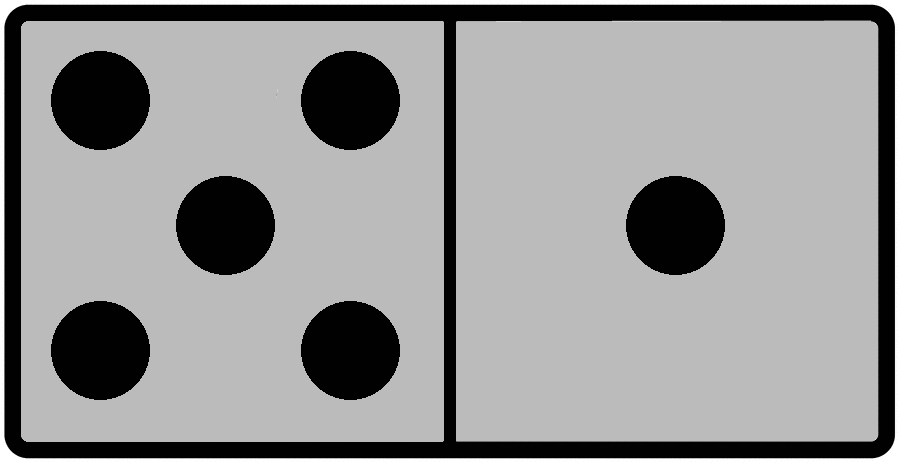
\includegraphics[width=0.2\textwidth]{gray5_1.png}}
\hspace{.1in}
\raisebox{-0.3\height}{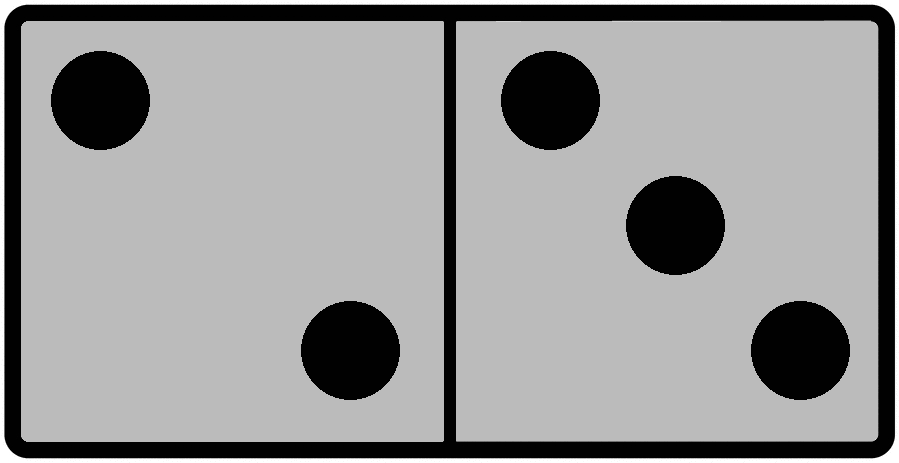
\includegraphics[width=0.2\textwidth]{gray2_3.png}}

Goal domino:
\hspace{1.1in}
\raisebox{-0.3\height}{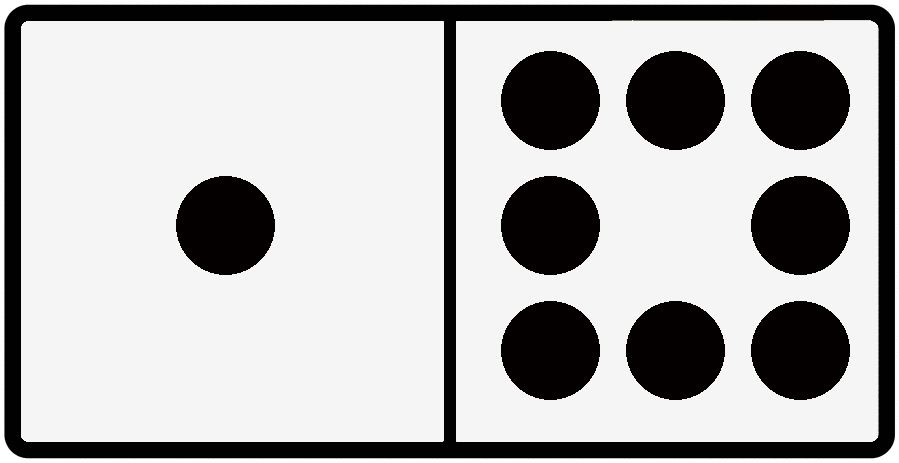
\includegraphics[width=0.2\textwidth]{white1_8.png}}

\footnotesize
(Hint: you may, if you wish, take ``a \textit{negative} number'' of one of the
dominoes. In other words, you can multiply the entire domino by a negative
number and then add it to your multiples of the other one.)
\normalsize

\item Starter dominoes:
\hspace{.3in}
\raisebox{-0.3\height}{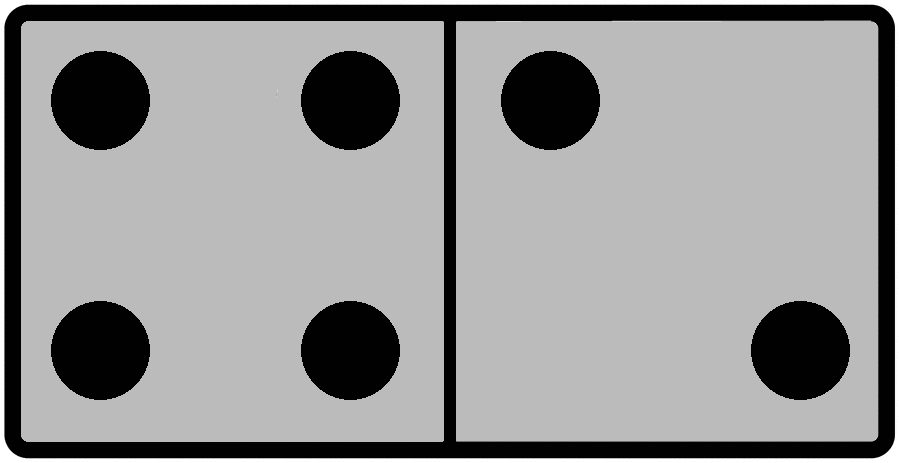
\includegraphics[width=0.2\textwidth]{gray4_2.png}}
\hspace{.1in}
\raisebox{-0.3\height}{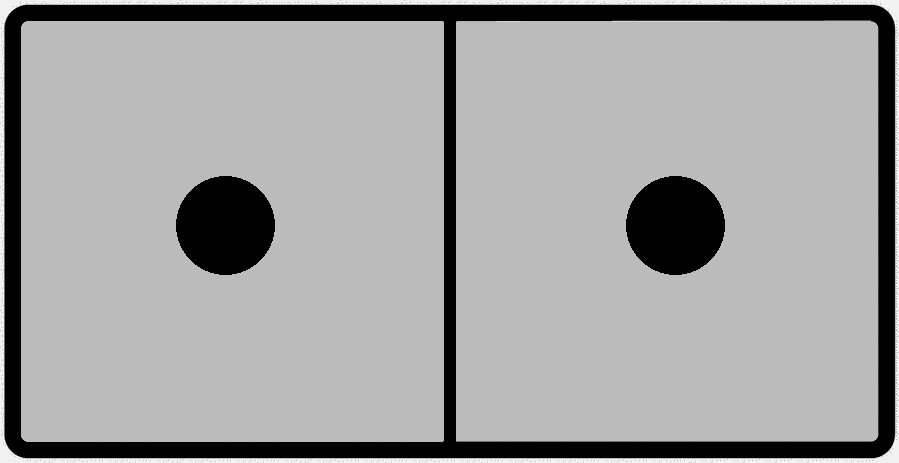
\includegraphics[width=0.2\textwidth]{gray1_1.png}}

Goal domino:
\hspace{1.1in}
\raisebox{-0.3\height}{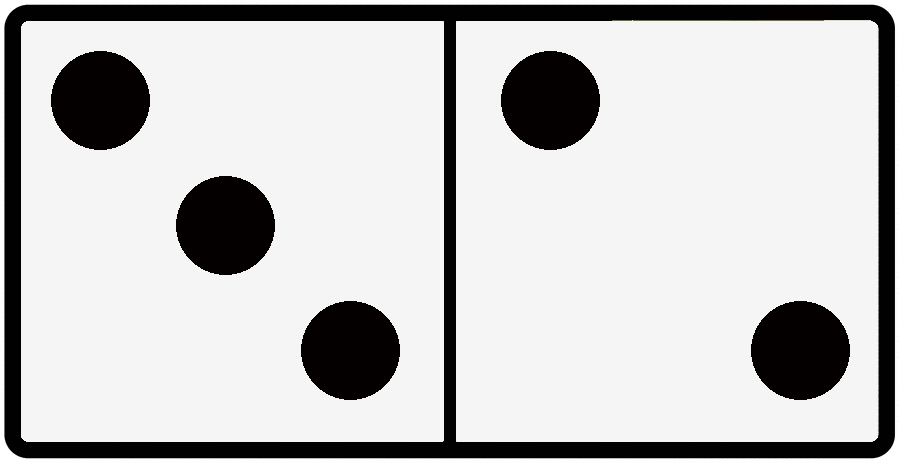
\includegraphics[width=0.2\textwidth]{white3_2.png}}

\footnotesize
(Hint: you can even take a \textit{fraction} of a domino, provided you take the
same fraction of both left and right sides. This means that just as you can
multiply an entire domino by a positive or negative number, or zero, you can
also multiply it by non-integers.)
\normalsize

\pagebreak
\item Starter dominoes:
\hspace{.3in}
\raisebox{-0.3\height}{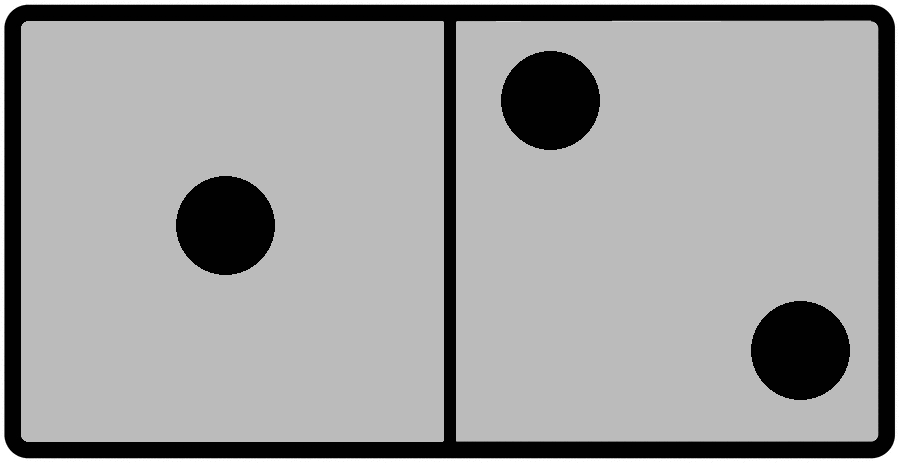
\includegraphics[width=0.2\textwidth]{gray1_2.png}}
\hspace{.1in}
\raisebox{-0.3\height}{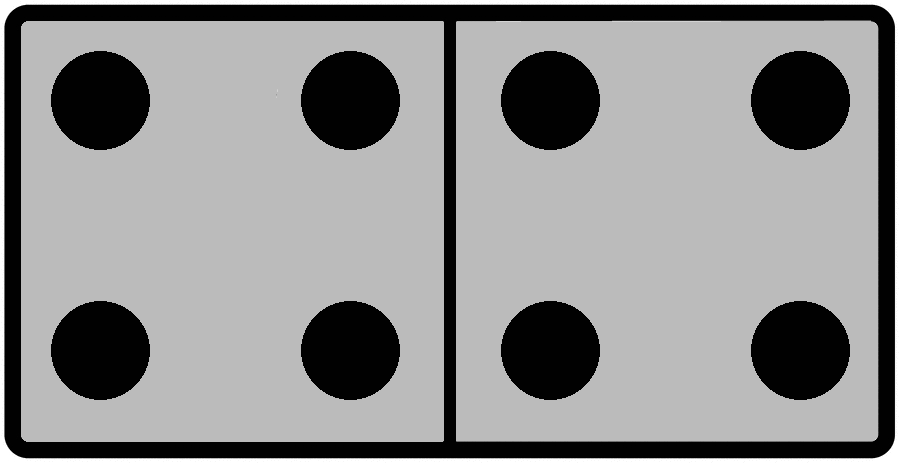
\includegraphics[width=0.2\textwidth]{gray4_4.png}}

Goal domino:
\hspace{1.1in}
\raisebox{-0.3\height}{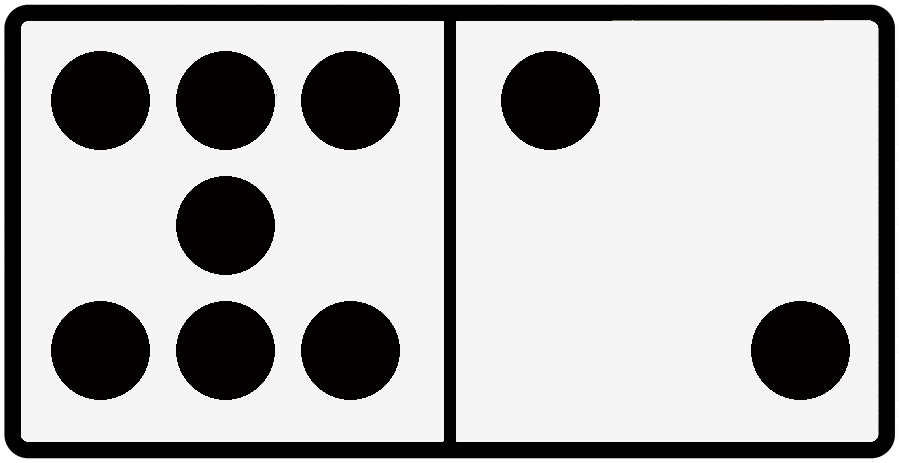
\includegraphics[width=0.2\textwidth]{white7_2.png}}

\footnotesize
(Hint: sometimes you have to go pretty far afield to get a solution, meaning a
large number of one domino and a large \textit{negative} number of the other.)
\normalsize

\item Starter dominoes:
\hspace{.3in}
\raisebox{-0.3\height}{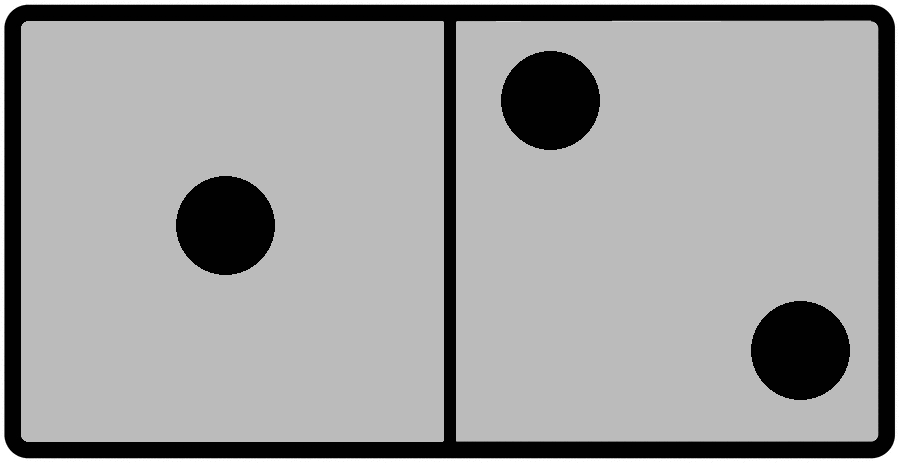
\includegraphics[width=0.2\textwidth]{gray1_2.png}}
\hspace{.1in}
\raisebox{-0.3\height}{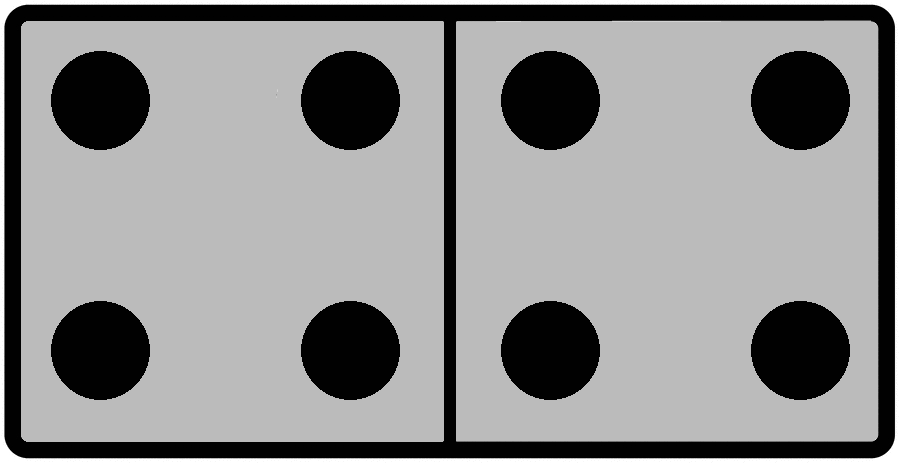
\includegraphics[width=0.2\textwidth]{gray4_4.png}}

Goal domino:
\hspace{1.1in}
\raisebox{-0.3\height}{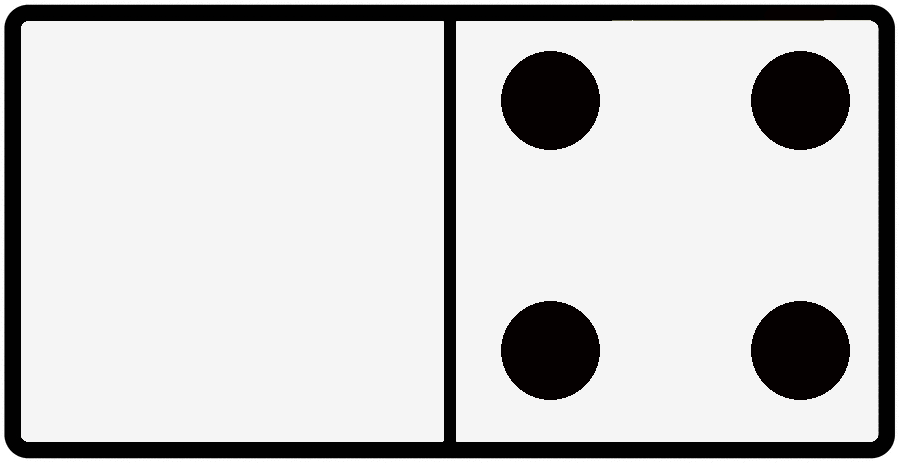
\includegraphics[width=0.2\textwidth]{white0_4.png}}

\footnotesize
(Hint: the goal domino can have a zero on it, just like the starter dominoes
did. But it's really no different; you just have to think creatively about how
to get the numbers to add up to zero on that side.)
\normalsize

\item Starter dominoes:
\hspace{.3in}
\raisebox{-0.3\height}{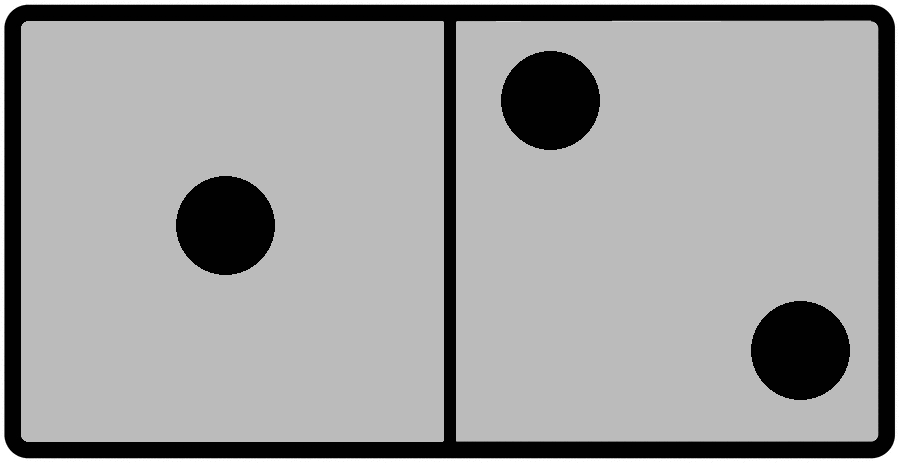
\includegraphics[width=0.2\textwidth]{gray1_2.png}}
\hspace{.1in}
\raisebox{-0.3\height}{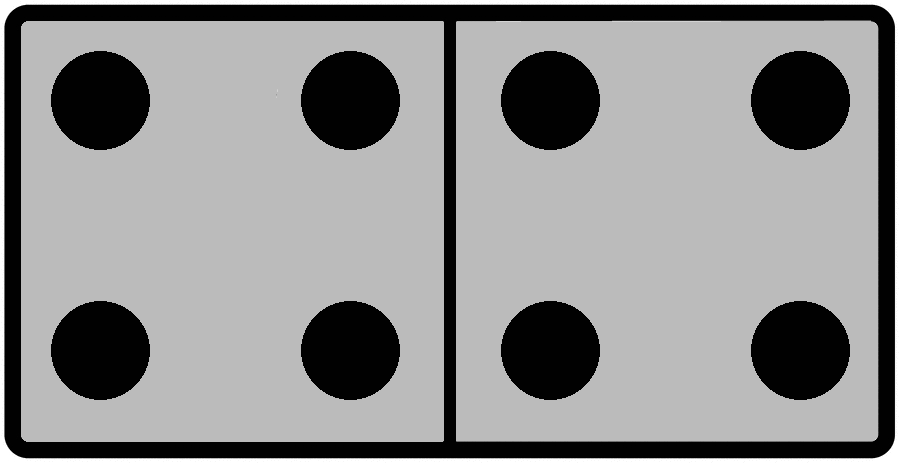
\includegraphics[width=0.2\textwidth]{gray4_4.png}}

Goal domino:
\hspace{1.1in}
\raisebox{-0.3\height}{
\includegraphics[width=0.2\textwidth]{white0_0.png}}

\footnotesize
(Hint: and yeah, the goal domino might even be \textit{completely} zero. That's
really not any different either, and in fact the solution will probably just
jump right off the page at you.)
\normalsize
\label{endDominoPuzzes}
\end{enumerate}

\bigskip
\subsection{Questions for curious minds}

I presume you have tried, and hopefully succeeded at most of these puzzles by
trial and error. Even if you didn't, I hope you've looked at and understood the
solutions I gave at the end of the chapter (p.~\pageref{dominoPuzzleAnswers}).

It's well worth taking a moment after all that fiddling around to consider some
interesting questions:

\begin{enumerate}
\itemsep.1em

\item \label{uniqueSolution} Were your solutions that same as mine in each
case? If so, do you think that was just coincidence? If not, how many different
solutions do you think are possible?

\item \label{alwaysSolveNoMatterGoal} Is it always possible to solve a puzzle
like this, no matter what the \textit{goal} domino is? Or are only a small
number of goal dominoes actually possible to produce?

\item \label{alwaysSolveNoMatterStarters} Is it always possible to solve a
puzzle like this, no matter what the \textit{starter} dominoes are? Or is it
only in a few cleverly crafted scenarios where the numbers happen to work out
just right?

\end{enumerate}

These matters turn out to be at the heart of the subject of linear algebra.
We'll shed light on all of them as we move forward.


\section{The Domino Game, Redux}

I'm now going to give you one more domino puzzle, which is going to seem at
first just like the others. But it turns out that hidden inside is a mystery, a
paradox, a conundrum that will shake our foundations in chapters to come. Here
it is:

\label{blueDominos}
Starter dominoes:
\hspace{.3in}
\raisebox{-0.3\height}{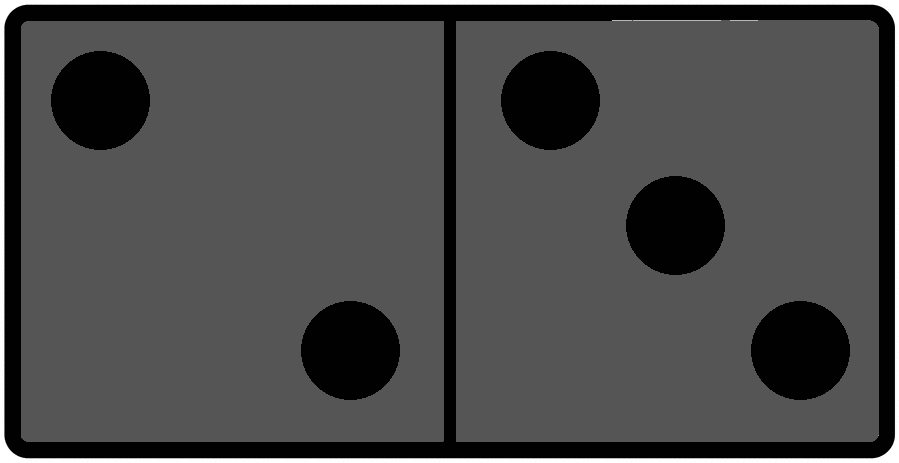
\includegraphics[width=0.3\textwidth]{darkgray2_3.png}}
\hspace{.1in}
\raisebox{-0.3\height}{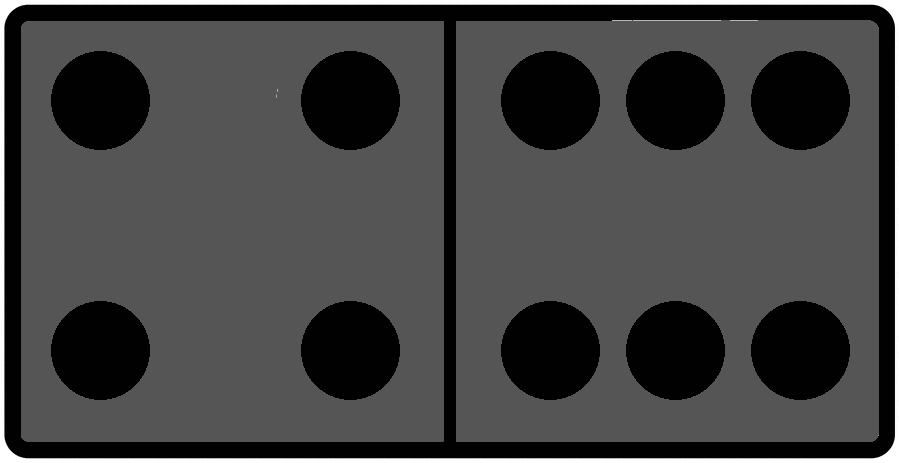
\includegraphics[width=0.3\textwidth]{darkgray4_6.png}}

Goal domino:
\hspace{1.3in}
\raisebox{-0.3\height}{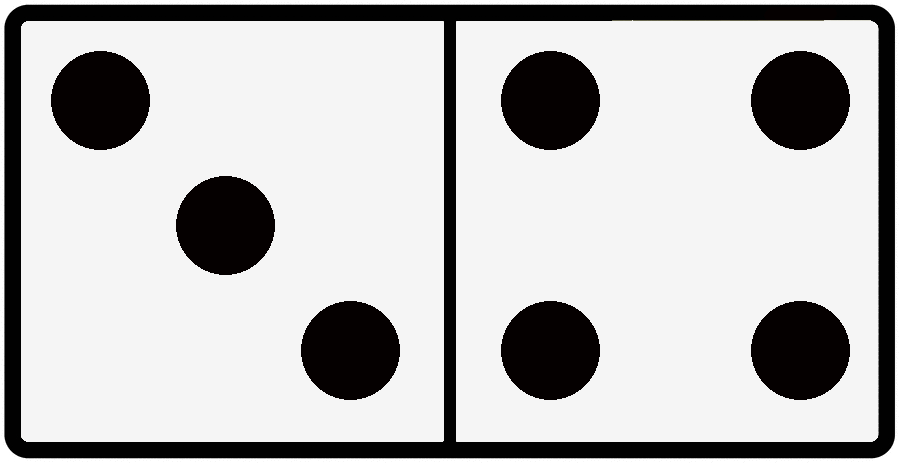
\includegraphics[width=0.3\textwidth]{white3_4.png}}

Our starter dominoes are \textbf{blue}\footnote{Dark gray, actually, since I
made this book black\&white to keep costs down.} instead of yellow this time,
for reasons I'll explain below. Other than that, it's the same kind of problem.
Go ahead -- try it!

I'll mail you \$5 if you can figure it out and send me a solution.

Actually, I'll make it \$5,000.

Don't get too frustrated before you realize the simple truth: it's not
possible.

\subsection{The key point: \underline{\textit{why}} blue dominoes don't work}

You don't have to be too clever to recognize that this whole Domino Game thing
is really math in disguise. And if you haven't seen the connection yet, let me
just point out the following so you can do a face palm:

\begin{compactitem}
\item Dominoes are just two-dimensional vectors.
\item ``Taking some number of the left (or right) domino'' is just
scalar-vector multiplication.
\item Adding together your copies-of-the-left-domino and your
copies-of-the-right-domino is just vector addition.
\end{compactitem}

\index{linear combination}
The central theme of the game is figuring out ``which vectors you can make from
which other vectors.'' The result of ``making'' a new domino is called a linear
combination:

\begin{center}
You get a \textbf{linear combination} of vectors when you multiply each of them
by a scalar and add them up (to yield another vector).
\end{center}

Any vector you can obtain this way is a linear combination of the vectors you
used. The scalars definitely don't have to all be the same. Also, each scalar
can be zero or even negative.

A critical question will turn out to be: what is the complete set of vectors
that are \textit{possible} to get as linear combinations of some ``starter
vectors?'' And to answer that, I'm going to give you a whole new perspective on
dominoes.

\subsection{Dominoes are vectors}

Several of our puzzles involved the yellow starter dominoes 1--2 and 4--4. As I
indicated, dominoes are really vectors in disguise. So I have plotted these two
``dominoes'' in Figure~\ref{fig:yellowVectors}.

\begin{figure}[ht]
\centering
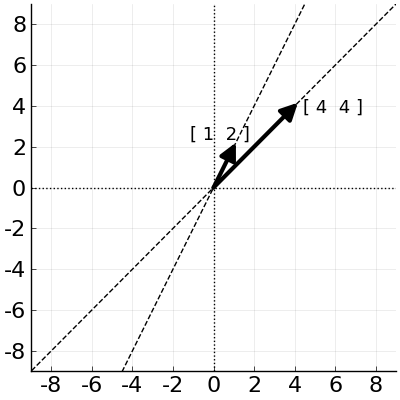
\includegraphics[width=0.8\textwidth]{yellowVectors.png}
\caption{Plotting the dominoes
\protect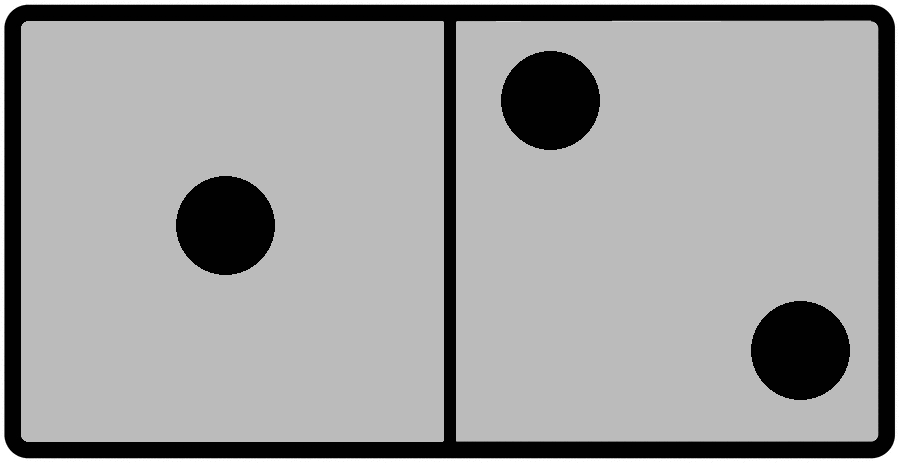
\includegraphics[width=0.07\textwidth]{gray1_2.png} and
\protect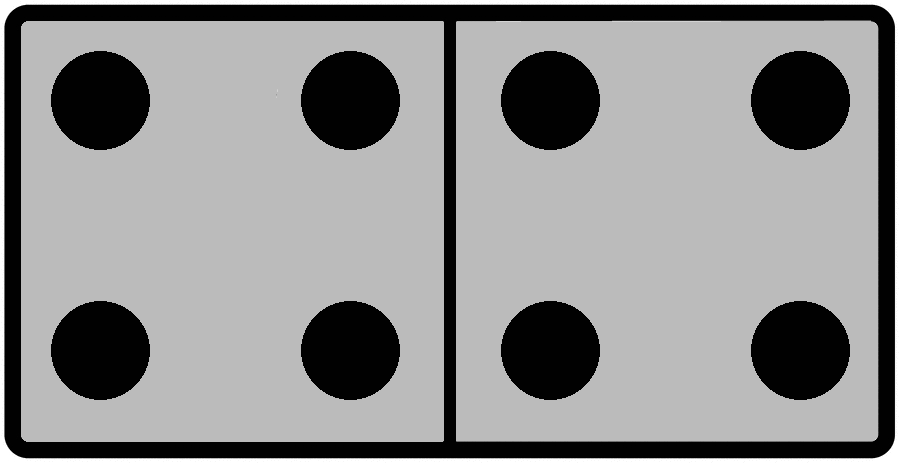
\includegraphics[width=0.07\textwidth]{gray4_4.png} as vectors.}
%\protect{\raisebox{-0.3\height}{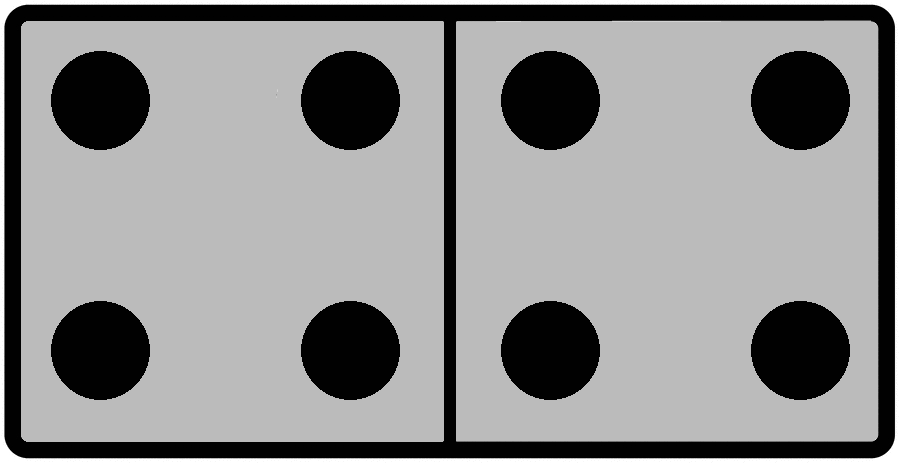
\includegraphics[width=0.05\textwidth]{gray4_4.png}}} as
%vectors.}
\label{fig:yellowVectors}
\end{figure}

Also on the diagram are two dashed lines, each going off to infinity in both
directions. Consider first the steepest of the two lines. It's pointing in
exactly the same direction as the $[\ 1\ \ 2\ ]$ vector. It represents
\textit{all the points you can get to by multiplying that vector by a scalar}.
Take a moment and digest that thought completely. You'll see that some of the
points that dashed line goes through are $(2,4)$, $(4,8)$, $(0,0)$,
$(-\frac{1}{2},-1)$, and $(-4,-8)$. Those points are the tips of the vectors
you would get if you multiplied $[\ 1\ \ 2\ ]$ by 2, 4, 0, $-\frac{1}{2}$, and
$-4$, respectively. Similar comments apply to the dashed line that extends the
$[\ 4\ \ 4\ ]$ vector.

Now consider the process of trying to reach a goal domino like
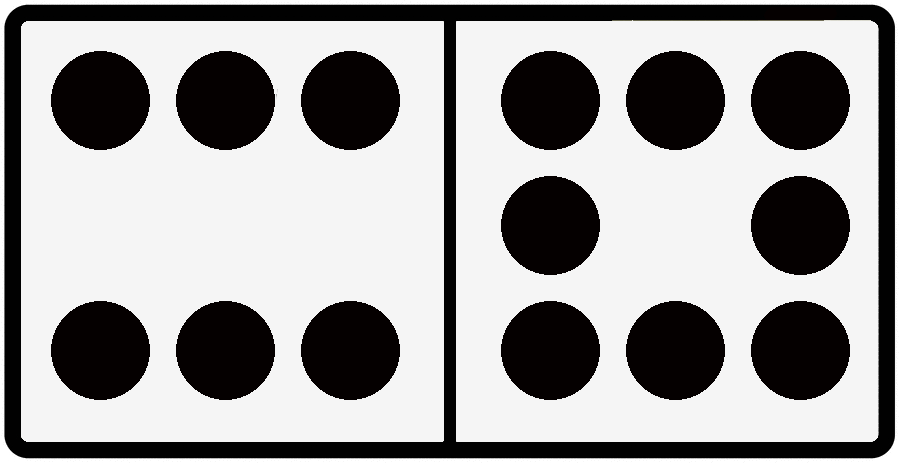
\includegraphics[width=0.06\textwidth]{white6_8.png}, also known as $[\ 6\ \ 8\
]$. What we're effectively asking is: is there any linear combination of $[\ 1\
\ 2\ ]$ and $[\ 4\ \ 4\ ]$ that will reach the point $[\ 6\ \ 8\ ]$? The
setting for this problem is on the left-hand side of 
Figure~\ref{fig:yellowVectors6_8}.

\begin{figure}[ht]
\centering
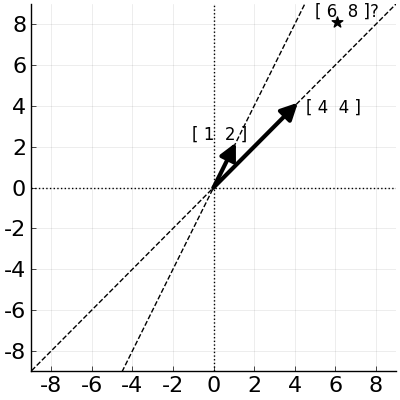
\includegraphics[width=0.44\textwidth]{yellowVectors6_8.png}
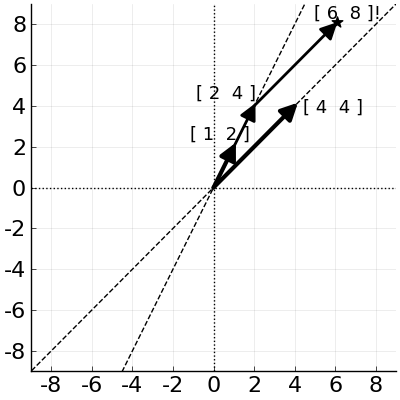
\includegraphics[width=0.44\textwidth]{yellowVectors6_8sol.png}
\caption{Can we reach the point
\protect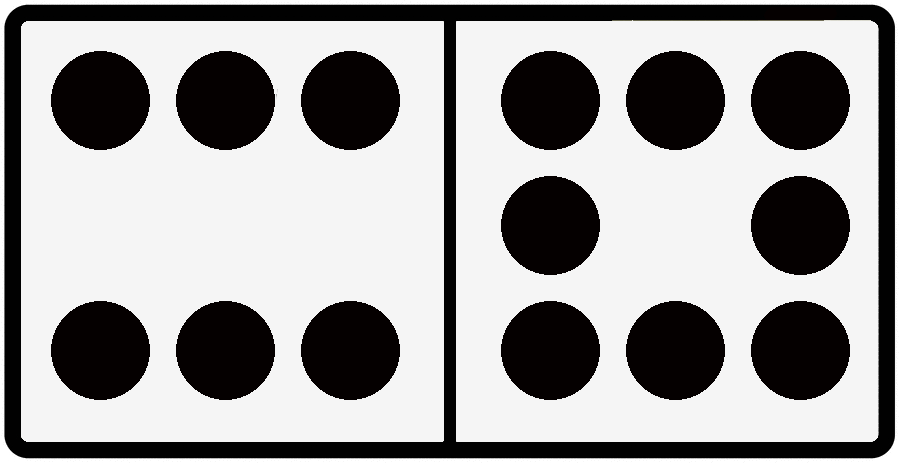
\includegraphics[width=0.06\textwidth]{white6_8.png} (the {\Large
$\star$} at
point $[\ 6\ 8\ ]$) using only multiples of the vectors
\protect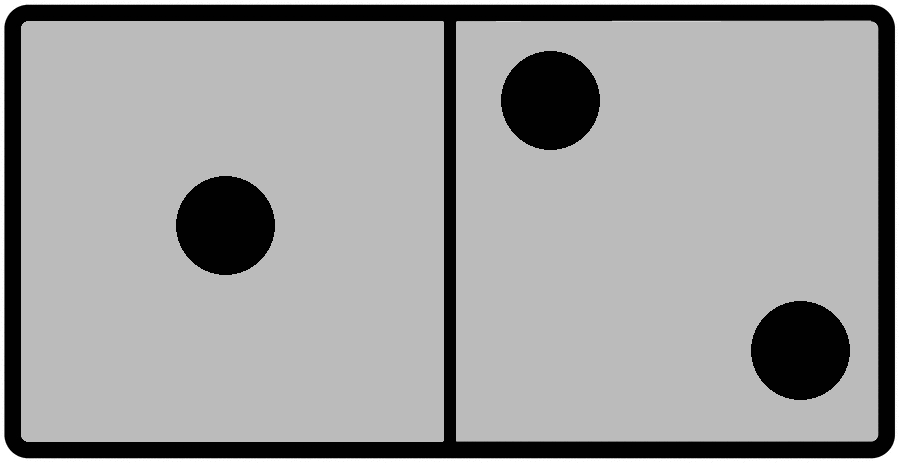
\includegraphics[width=0.06\textwidth]{gray1_2.png} and
\protect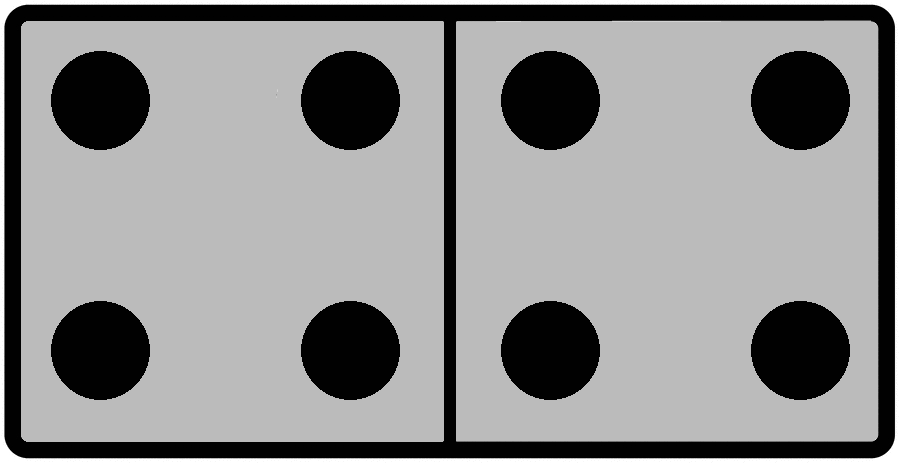
\includegraphics[width=0.06\textwidth]{gray4_4.png}? \textit{Yes!}}
\label{fig:yellowVectors6_8}
\end{figure}

By fiddling around with these numbers Domino-Game-style, you'll hit on the
solution of ``\textbf{two} and \textbf{one}'': two
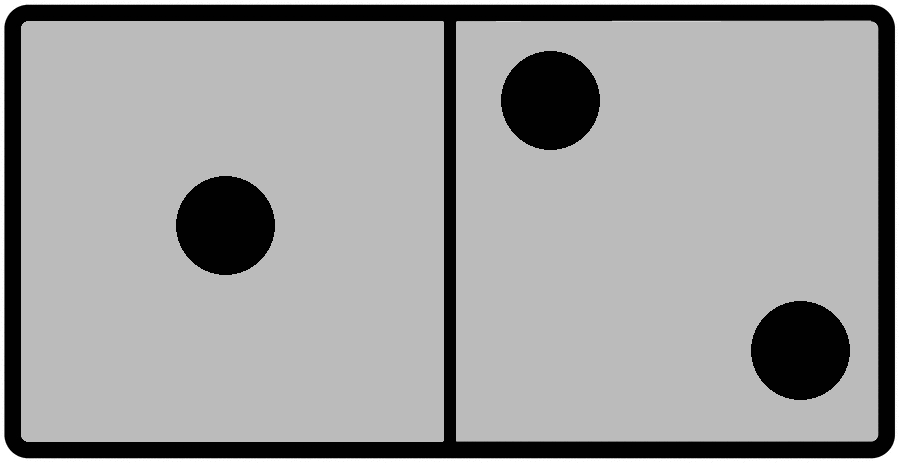
\includegraphics[width=0.06\textwidth]{gray1_2.png} dominoes plus one
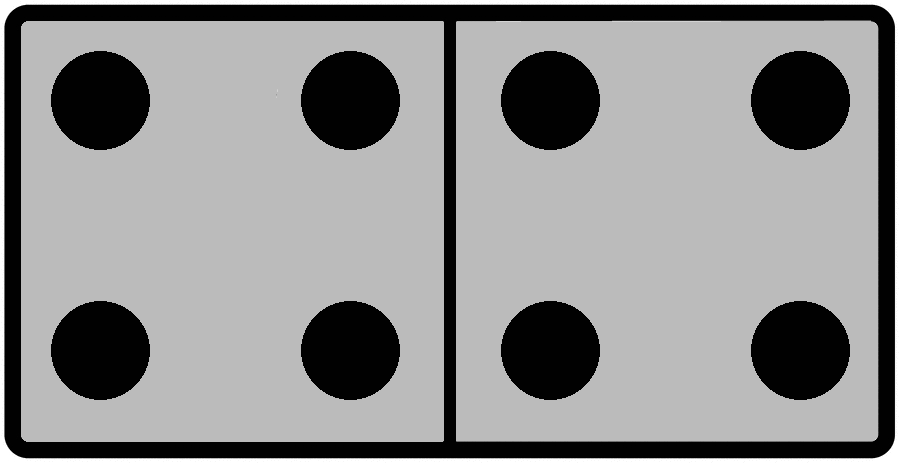
\includegraphics[width=0.06\textwidth]{gray4_4.png} domino gives you a
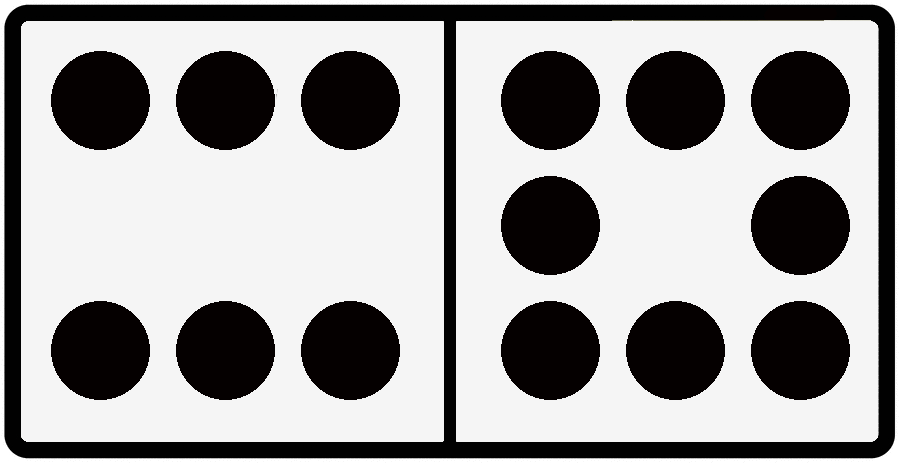
\includegraphics[width=0.06\textwidth]{white6_8.png} domino. That can be
pictured visually on the right-hand side Figure~\ref{fig:yellowVectors6_8}.
Starting at the origin, and moving two times in the direction of the $[\ 1\ \
2\ ]$ vector, we get to the point $[\ 2\ \ 4\ ]$. From there, moving once in
the direction of the $[\ 4\ \ 4\ ]$ vector lands us exactly on the point $[\ 6\
\ 8\ ]$. Voil\`{a}!

\medskip

That was fun -- let's try some more. What about the point $[\ 3\ \ 2\ ]$. Can
we reach \textit{it} by using only multiples of $[\ 1\ \ 2\ ]$ and $[\ 4\ \ 4\
]$?

\index{windshield wiper}
At first glance, it doesn't seem so; after all, the point $(3,2)$ is outside
the ``windshield wiper'' angle between the two dashed lines. But it turns out
we can, if we go against the grain. Moving ``$-1$ times in the $[\ 1\ \ 2\ ]$
direction'' takes us to the point $[\ -1\ \ -2\ ]$. From there, we do
\textit{almost} a complete 180\textdegree. Heading back northeast once in the
$[\ 4\ \ 4\ ]$ direction lands us on $[\ 3\ \ 2\ ]$ as desired. Bingo! (See
Figure~\ref{fig:yellowVectors3_2}.)

\begin{figure}[ht]
\centering
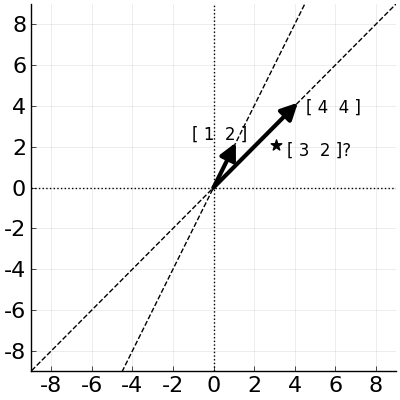
\includegraphics[width=0.44\textwidth]{yellowVectors3_2.png}
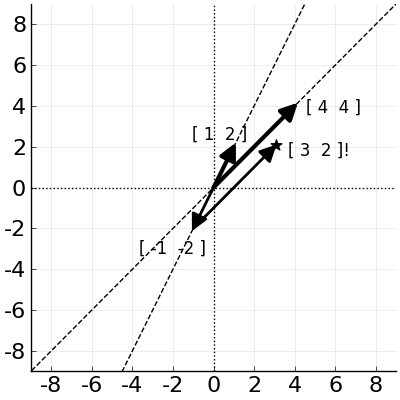
\includegraphics[width=0.44\textwidth]{yellowVectors3_2sol.png}
\caption{Can we reach the point $[\ 3\ \ 2\ ]$ using only $[\ 1\ \ 2\ ]$ and
$[\ 4\ \ 4\ ]$? \textit{Yes!}}
\label{fig:yellowVectors3_2}
\end{figure}

\index{backwards}
And how about $[\ 0\ \ 4\ ]$? This time it's the 
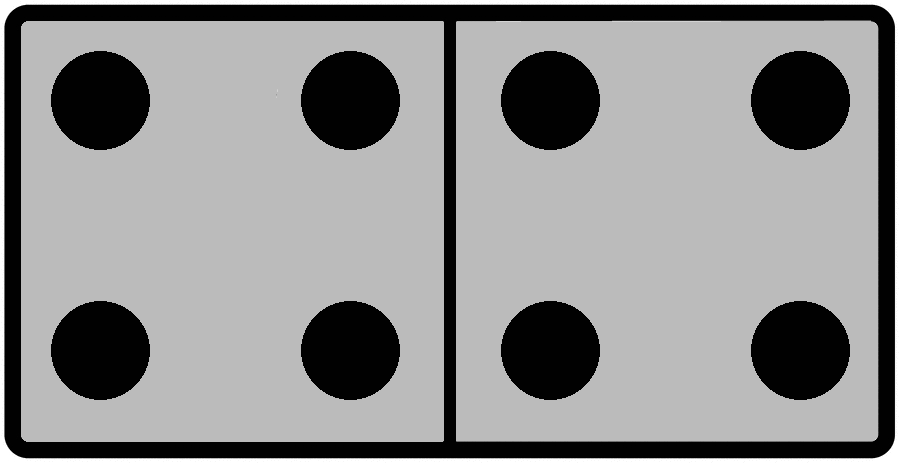
\includegraphics[width=0.06\textwidth]{gray4_4.png} domino that we use
``backwards.'' Going four times in the $[\ 1\ \ 2\ ]$ direction followed by
$-1$ in the $[\ 4\ \ 4\ ]$ direction gives us the solution ``4 \& $-1$,'' as
depicted in Figure~\ref{fig:yellowVectors0_4}.

\begin{figure}[hb]
\centering
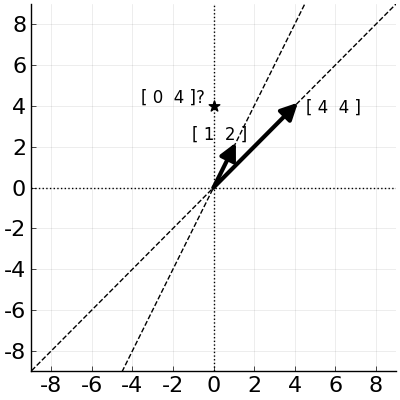
\includegraphics[width=0.44\textwidth]{yellowVectors0_4.png}
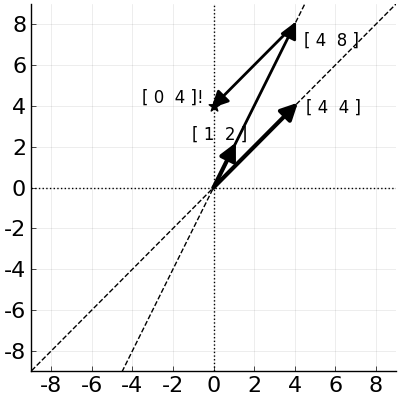
\includegraphics[width=0.44\textwidth]{yellowVectors0_4sol.png}
\caption{Can we reach the point $[\ 0\ \ 4\ ]$ using only $[\ 1\ \ 2\ ]$ and
$[\ 4\ \ 4\ ]$? \textit{Yes!}}
\label{fig:yellowVectors0_4}
\end{figure}

At this point, you'll probably guess what I'm going to say next. Yes indeed,
\textit{any} point in the entire $x,y$ plane can be reached through some
combination of the $[\ 1\ \ 2\ ]$ and $[\ 4\ \ 4\ ]$ vectors. And that gives us
the answer to one of our questions from p.~\pageref{alwaysSolveNoMatterGoal}
(question \#\ref{alwaysSolveNoMatterGoal}): surprisingly, \textit{yes} we can
always find a solution to the Domino Game puzzle, no matter what the goal
domino is. Amazing!

Most of my students are as surprised by that result as I was back in the day.
When I first give them Domino puzzles, they figure, ``okay, Stephen has
specially concocted a case where it just happens to work out that I can combine
the two yellow dominoes into a white one somehow. I'll work his special puzzle
and come up with the slick answer.'' Little do they realize that \textit{any}
white domino whatsoever is solvable; I didn't have to come up with anything
special at all.

\smallskip

Now the second lesson of these vector pictures may be harder to see. It's the
answer to question \#\ref{uniqueSolution} from p.~\pageref{uniqueSolution}. Not
only can every Domino problem be solved, but \textit{it can be solved in only
one way.}

If you did it right, your answers to the six puzzles on
pp.~\pageref{startDominoPuzzles}-\pageref{endDominoPuzzes} were exactly the
same as mine on p.~\pageref{dominoPuzzleAnswers}. Perhaps that struck you as a
coincidence at first: ``gee, it's sure funny that I always keep hitting on the
exact same solution that Stephen did!'' But if you stare at
Figure~\ref{fig:yellowVectors6_8} and friends, you might see the reason.
Starting from the origin, and striking out in the first vector's direction, you
only have one choice if you want to get to the right place. In
Figure~\ref{fig:yellowVectors6_8}'s case, you \textit{must} stop at $[\ 2\ \ 4\
]$. If you stop earlier, or later, then you're destined to miss the mark: going
in the $[\ 4\ \ 4\ ]$ direction from anywhere else you might stop won't land
you at exactly $[\ 6\ \ 8\ ]$.

\subsection{But...}

So every point is reachable, and is reachable in only one way. But that's only
\textit{\underline{if}} you have yellow starter dominoes. If you've got blue
ones, it's a totally different story.

\begin{figure}[ht]
\centering
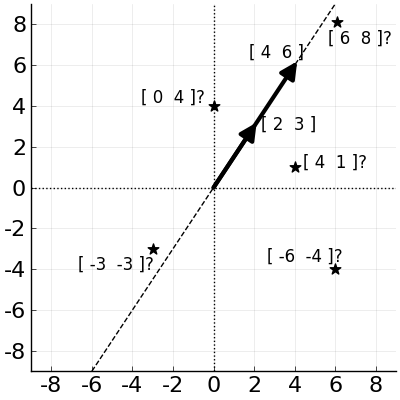
\includegraphics[width=0.7\textwidth]{blueVectors.png}
\caption{Can we reach the points
$[\ 6\ \ 8\ ]$,
$[\ 0\ \ 4\ ]$,
$[\ 4\ \ 1\ ]$,
$[\ -6\ \ -4\ ]$,
$[\ -3\ \ -3\ ]$...or virtually anything else
using only $[\ 2\ \ 3\ ]$ and $[\ 4\ \ 6\ ]$? \textbf{No.}}
\bigskip
\label{fig:blueVectors}
\end{figure}

Figure~\ref{fig:blueVectors} shows the hopeless situation. The telltale sign of
misery is that \textit{there's only one dashed line.} The 
{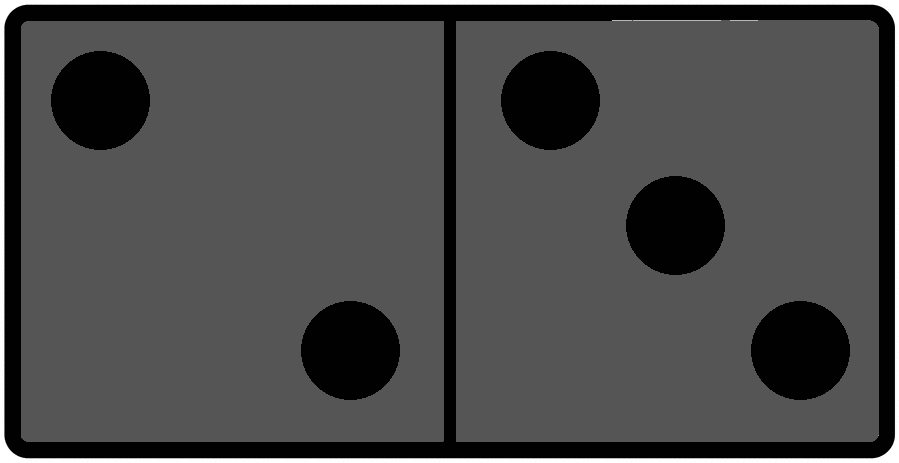
\includegraphics[width=0.06\textwidth]{darkgray2_3.png}} and
{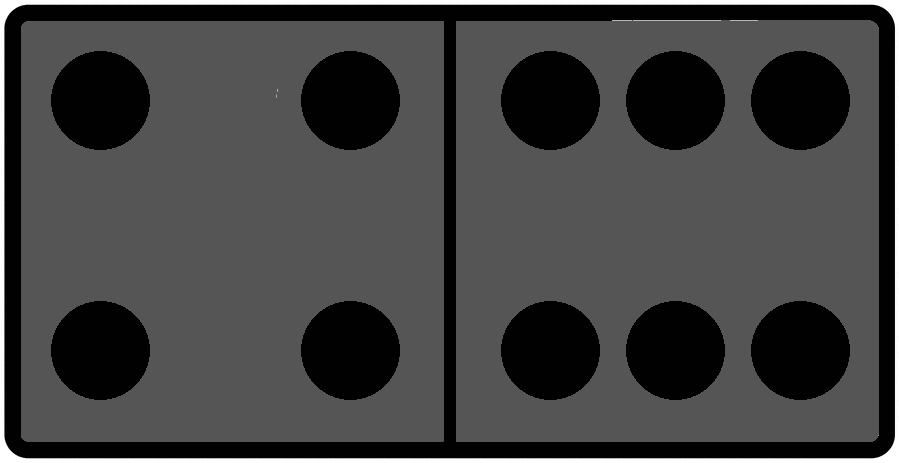
\includegraphics[width=0.06\textwidth]{darkgray4_6.png}} vectors point in
\textit{exactly} the same direction, so no matter how hard we try, there's no
getting off that one line. In the middle of a promising two-dimensional
landscape, we're stuck in a one-dimensional sub-world.


\section{Linear independence in two dimensions}

\index{linear independence}

The yellow {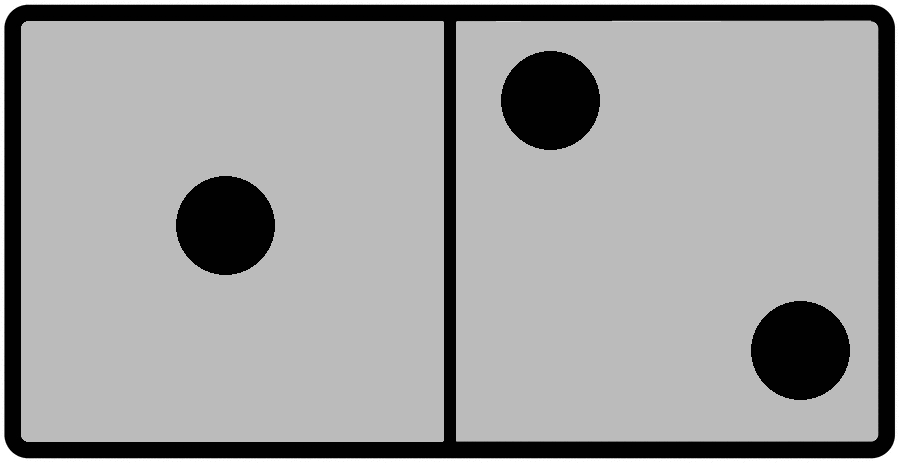
\includegraphics[width=0.06\textwidth]{gray1_2.png}} and
{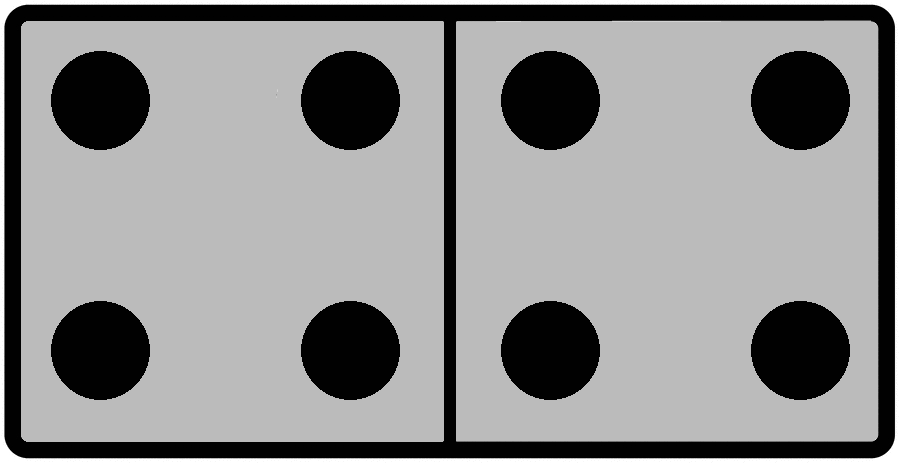
\includegraphics[width=0.06\textwidth]{gray4_4.png}} vectors are called
\textbf{linearly independent}. By contrast, the blue
{\includegraphics[width=0.06\textwidth]{darkgray2_3.png}} and
{\includegraphics[width=0.06\textwidth]{darkgray4_6.png}} vectors are
\textbf{linearly dependent}. Figure~\ref{fig:dominoFacts}
(p.~\pageref{fig:dominoFacts}) sums up some
extremely important facts about these two cases in one handy table. Let me
explain each item in turn.

\vspace{-.2in}

\begin{itemize}
\itemsep.1em

\item \textbf{Yellow dominoes are linearly independent.} This means they point
in different directions, so that each one gives you a ``fresh'' degree of
freedom to travel in.

% DANGER: "up" to refer to figure

\item \textbf{You can't get one yellow domino from the other.} A corollary of
the ``different directions'' thing is that if you tried to get to the tip of
the first yellow domino using only the second, you couldn't do it. Look back at
Figure~\ref{fig:yellowVectors} (p.~\pageref{fig:yellowVectors}) if you don't
believe me. From the origin, can you get to the point $[\ 1\ \ 2\ ]$ going only
in the $[\ 4\ \ 4\ ]$ direction? No. But if you look up at
Figure~\ref{fig:blueVectors} you'll see that you \textit{can} do it with our
blue dominoes. Can you get to $[\ 2\ \ 3\ ]$ using only the $[\ 4\ \ 6\ ]$
vector? Sure, just take half of it.

Another way to think of it is that if you have blue dominoes, one of them is
superfluous. Say you have $[\ 2\ \ 3\ ]$, and I come along trying to sell you
$[\ 4\ \ 6\ ]$ as well. Why bother? You can already go in that direction! Heck,
you can produce $[\ 4\ \ 6\ ]$ yourself just by doubling the domino you already
have.


\item \textbf{Yellow dominoes are the common case.} Suppose I picked two
dominoes out of a bag and put them in front of you. Are they more likely to be
yellow, or blue? A moment's consideration will tell you the answer is yellow.
The only way the dominoes can be blue is if they point in
\underline{\textit{exactly}} the same direction. The odds of that are
fantastically small.

Think of it this way. Let's say the first domino out of the bag is $[\ 1\ \ 3\
]$. And let's say the left half of the second domino is 4, so that the second
domino is $[\ 4\ \ ?\ ]$. Think about what would have to happen for the pair of
dominoes to be blue. That question mark would have to be exactly 12.
\textit{Only} 12. Absolutely any other number for the question mark would give
you yellow dominoes.

\item \textbf{With yellow dominoes, you can get \textit{any} white domino.}
This is perhaps the most important point. The yellow dominoes have enough
coverage that any point in the entire plane is reachable using them. The sorry
blue dominoes, on the other hand, are inbred; you can't get anywhere on the
plane except the points along their shared, lonely line.

\item \textbf{With yellow dominoes, each solution is unique.} This may or may
not have been obvious to you from the diagrams, but I promise it's so. You can
reach each point in only one way. By contrast, everything the blue dominoes can
reach -- which admittedly, ain't much -- can be reached in multiple ways
(including the origin; see the next point).

\index{trivial@``trivial'' solution}

\item \textbf{Yellow dominoes can't get to the origin, except ``trivially.''}
One last point is that with yellow dominoes, the only way to get to the origin
is to take zero of the first domino and zero of the second. (This is called a
\textbf{trivial solution}.) That's because once you set out in the first
domino's direction, using the second one has to take you in a
\textit{different} direction, and hence not back to where you came. With blue
dominoes, you can do this in many different ways: take six $[\ 2\ \ 3\ ]$'s
minus three $[\ 4\ \ 6\ ]$'s, or $-1$ $[\ 2\ \ 3\ ]$'s and half a $[\ 4\ \ 6\
]$, \textit{etc.} I guess that's some small recompense for having to stay on
that one line: blue dominoes truly \textit{own} that line and can tread it to
their heart's content. This seemingly obscure fact will actually play a
surprising role later on.

\end{itemize}

By the way, a student once asked me, ``what if you get one yellow domino and
one blue? What happens then?'' Perhaps you'll see the answer immediately as one
of my other students did. The answer is \textit{that can't happen.} No domino
is, by itself, intrinsically yellow or blue: it's only yellow or blue
\textit{with respect to another one.} It's the \textit{pair} of dominoes that
are yellow if they point in different directions, or blue if they point in the
same direction.


\begin{figure}[ht]
\begin{framed}
\begin{center}
\small
\hspace{-.2in}
\begin{tabular}{l|r}
Yellow dominos \ 
\raisebox{-0.25\height}{\includegraphics[width=0.07\textwidth]{gray1_2.png}} 
\raisebox{-0.25\height}{\includegraphics[width=0.07\textwidth]{gray4_4.png}} &
\raisebox{-0.25\height}{\includegraphics[width=0.07\textwidth]{darkgray2_3.png}} 
\raisebox{-0.25\height}{\includegraphics[width=0.07\textwidth]{darkgray4_6.png}} 
\ Blue dominos \smallskip \\
\hline \\ 
linearly \textbf{independent} & linearly \textbf{dependent} \\
can't get any yellow from others & 
can get each blue from others \\
``common'' & ``rare'' \\
can make \textit{any} white domino & can make only a few \\
each goal reachable in one way & each goal reachable \textit{many} ways \\
can only get
\raisebox{-0.3\height}{\includegraphics[width=0.07\textwidth]{white0_0.png}} 
``trivially" &
can get 
\raisebox{-0.3\height}{\includegraphics[width=0.07\textwidth]{white0_0.png}}
in many ways \\
\end{tabular}
\end{center}
\end{framed}
\vspace{-.2in}
\caption{Important domino facts.}
\label{fig:dominoFacts}
\end{figure}

% linearly dependent: can get to zero non-trivially, and to any point on the
%   line in multiple ways
% linearly dependent is rarer
% you can't have "one blue domino"

\pagebreak
\subsection*{Answers to Domino Game puzzles from
pp.~\pageref{startDominoPuzzles}-\pageref{endDominoPuzzes}}
\label{dominoPuzzleAnswers}

\begin{enumerate}
\itemsep1em

\item {Solution: \textbf{0 \& 2}}

\quad 0 \raisebox{-0.3\height}{\includegraphics[width=0.1\textwidth]{gray5_1.png}} \ \& \
2 \raisebox{-0.3\height}{\includegraphics[width=0.1\textwidth]{gray2_3.png}} \ = \
\raisebox{-0.3\height}{\includegraphics[width=0.1\textwidth]{white4_6.png}} \quad

\item {Solution: \textbf{--1 \& 3}}

\ $-1$ \raisebox{-0.3\height}{\includegraphics[width=0.1\textwidth]{gray5_1.png}} \ \& \
3 \raisebox{-0.3\height}{\includegraphics[width=0.1\textwidth]{gray2_3.png}} \ = \
\raisebox{-0.3\height}{\includegraphics[width=0.1\textwidth]{white1_8.png}} \quad

\item {Solution: \textbf{$\frac{1}{2}$ \& 1}}

\quad $\frac{1}{2}$ \raisebox{-0.3\height}{\includegraphics[width=0.1\textwidth]{gray4_2.png}} \ \& \
1 \raisebox{-0.3\height}{\includegraphics[width=0.1\textwidth]{gray1_1.png}} \ = \
\raisebox{-0.3\height}{\includegraphics[width=0.1\textwidth]{white3_2.png}} \quad

\item {Solution: \textbf{-5 \& 3}}

\ $-5$ \raisebox{-0.3\height}{\includegraphics[width=0.1\textwidth]{gray1_2.png}} \ \& \
3 \raisebox{-0.3\height}{\includegraphics[width=0.1\textwidth]{gray4_4.png}} \ = \
\raisebox{-0.3\height}{\includegraphics[width=0.1\textwidth]{white7_2.png}} \quad

\item {Solution: \textbf{4 \& --1}}

\quad 4 \raisebox{-0.3\height}{\includegraphics[width=0.1\textwidth]{gray1_2.png}} \&
$-1$ \raisebox{-0.3\height}{\includegraphics[width=0.1\textwidth]{gray4_4.png}} \ = \
\raisebox{-0.3\height}{\includegraphics[width=0.1\textwidth]{white0_4.png}} \quad

\item {Solution: \textbf{0 \& 0}}

\quad 0 \raisebox{-0.3\height}{\includegraphics[width=0.1\textwidth]{gray1_2.png}} \ \& \
0 \raisebox{-0.3\height}{\includegraphics[width=0.1\textwidth]{gray4_4.png}} \ = \
\raisebox{-0.3\height}{\includegraphics[width=0.1\textwidth]{white0_0.png}} \quad

\end{enumerate}
